
\section{Integrability conditions and limitations of the pure mapping approach}

In a previous publication~\cite{Baeuerle2012}, the authors
presented a design algorithm for freeform optics that can handle
multiple optical surfaces whilst at the same time operating directly
with a prescribed target irradiance pattern.  The optical surfaces are
designed to be coupled to a zero-\'{e}tendue source (for example a point
source or a perfectly collimated source). Each source ray is uniquely
associated with a point in a 2D plane $\Omega_0$ perpendicular to the
optical axis via a suitable projection, creating a flux density
$\mu_0$ in this plane. The target irradiance is equally projected in a
consistent way onto a target plane $\Omega_1$ with density
$\mu_1$. The task of designing a (freeform) optical system then
amounts to finding a diffeomorphism (``ray mapping'') so that the
transformed irradiance distribution matches the target distribution:
\begin{equation}
  u:\Omega_0\to\Omega_1, (x,y)\mapsto(t_x,t_y)\text{~with~}\mu_0=|\mathrm{D}u|\mu_1\circ u
\end{equation}
Here, $(t_x,t_y)$ represents the target point in $\Omega_1$ to be
reached by a source ray passing through $(x,y)$ in $\Omega_0$ (see
Fig.~\ref{fig:1surf-setup}). $\mathrm{D}u$ is the Jacobian of $u$ and
$\circ$ refers to the standard composition operator.

An initial mapping $\tilde{u}$ between these two planes can easily be
computed using successive one-dimensional integrations along the
Cartesian coordinate axes~\cite{Parkyn1998}. In a second step, this
mapping is optimized to make it irrotational. Haker~\cite{Haker2004}
proposed an evolution equation over a pseudo-time variable $t$ towards
a stationary solution ($t~\to~\infty$):

\begin{equation}
  \pderiv{u}{t} = -\frac{1}{\mu_0} \; {\rm D} u\; \nabla^\bot \left( \Delta^{-1}\ddiv  u^\bot \right)\text{\quad with } \left.u\right|_{t=0}=\tilde{u}
  \label{eq:haker-ev}
\end{equation}
where $(x,y)^\bot~=~(-y,x)$ represents a rotation by 90~degrees in
$\mathbb{R}^2$ and $\Delta^{-1}\ddiv u^\bot$ denotes the solution $f$
of Poisson's equation $ \Delta f = -\ddiv u^\bot $.  The stationary
solution of this equation is the optimal mapping (for a quadratic cost
function) transforming the source density~$\mu_0$ into the target
density~$\mu_1$ and it is irrotational, which is the property of
interest here.

It is well established~\cite{Fournier2010,Ries2002} that a 3D vector
field of surface normals $\mathbf{N}$ represents a family of
continuous surfaces if and only if the so-called integrability
condition is satisfied:
\begin{equation}
  C = \N \cdot (\nabla \times \N) = 0
  \label{eq:integ}
\end{equation}
In the optical case at hand, this family is the set of Cartesian ovals
transforming the input wave front into the output wave-front.
This condition has the dimensions of the inverse of a length. The
integrability criterion on $\mathbf{N}$ is not strictly enforced
in~\cite{Baeuerle2012} and instead, a surface reconstruction is
proposed using a least-squares optimization that minimizes the
deviation of ray positions on the target (as found through numerical
ray tracing) from their positions as prescribed by the mapping.


\subsection{Collimated case}

We now show in detail why the curl-removal of the ray mapping (instead
of the normal field directly) proposed in~\cite{Baeuerle2012} and used
in~\cite{Bruneton2012} provides
a valid approximation to the full integrability
condition~\eqref{eq:integ}, and what are the limits of this
approximation.  The computations that follow only deal with the case
of a collimated source and one optical surface as shown in
Fig.~\ref{fig:1surf-setup} to maintain the clarity of the argument. 
A similar (but much longer) development can be performed for two optical
surfaces considering then the two successive light deflections.

\TODO figure d'Axel

\begin{figure}[!htbp]
  \centering 
  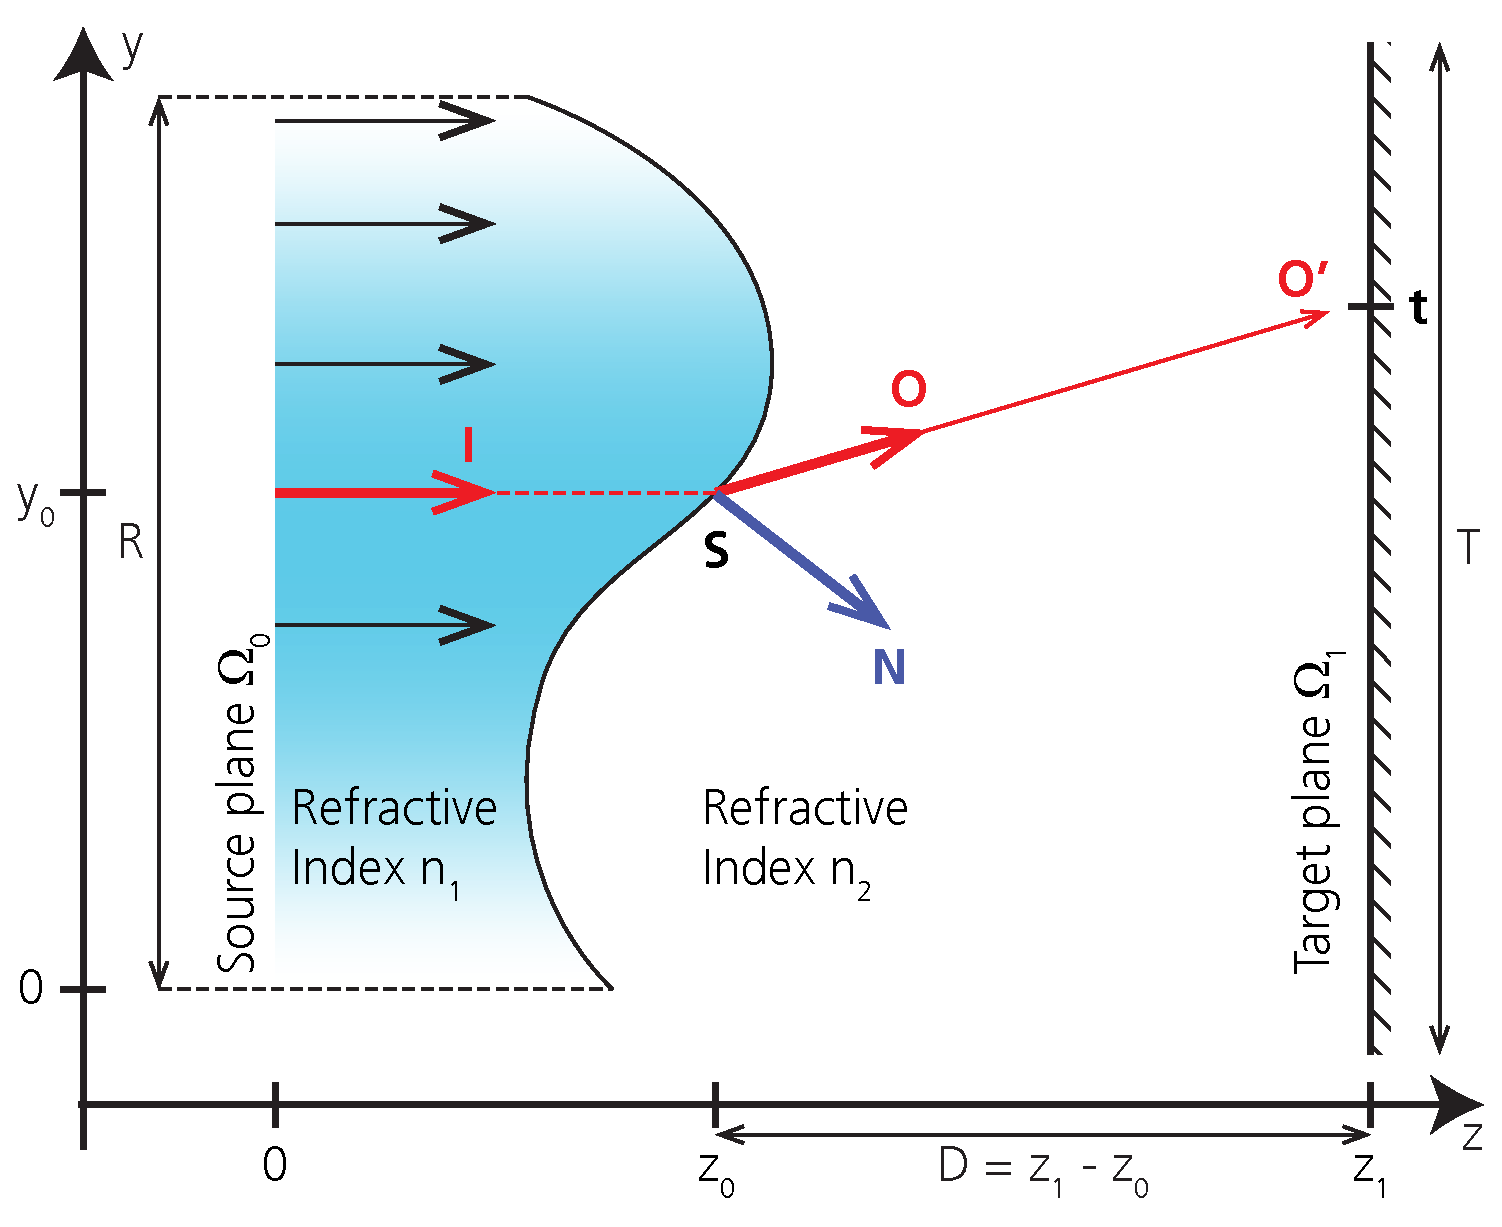
\includegraphics[width=0.49\textwidth]{geometrie_integ}
  \caption{Single-surface setup with a collimated source.}
  \label{fig:1surf-setup}
\end{figure}

Denoting $\I$ and $\OO$ the light incident and output unit vectors onto 
an optical surface with unit normal $\mathbf{N}$, one can write 
Snell's laws in a vectorial form\cite{Benitez2004b}:
\begin{equation}
  n_1 \mathbf{N} \times \mathbf{I} = n_2 \mathbf{N} \times \mathbf{O} 
  \label{eq:snell}
\end{equation}

From this, it follows that 
\[ \N=\Np\big/ \|\Np \|\text{~with~}\Np = n_1 \I - n_2 \OO,\]
Given a mapping $u$, the set of unit vectors $\I$ and $\OO$  can 
directly be seen as full 3D vector fields (by associating the vector supporting 
the ray to each point along the ray trajectory).
The integrability condition \eqref{eq:integ} applies equally to the non-normalized
vector field $\Np$, which yields:
\[ C = \left( n_1 \I - n_2 \OO \right) \cdot
       \left( n_1 \curl{\I} - n_2 \curl{\OO} \right) \]
This can be expanded into:
\begin{align*}
 C =\quad & n_1^ 2 \I\cdot(\curl{\I}) + n_2^2 \OO\cdot (\curl{\OO}) \nonumber \\
 & - n_1 n_2 ( \I \cdot (\curl{\OO}) + \OO\cdot (\curl{\I}))
\end{align*}

%In the setup considered here,
%the curl of the source rays is null, and hence $\I$ always 
%fulfills~\eqref{eq:integ}. 
Zero-\'{e}tendue ray bundles in homogeneous media (like our source) 
are always irrotational~\cite{Minano2004z}, and hence $\I$ always 
fulfills~\eqref{eq:integ}. 
With an irrotational mapping,
the output field $\OO$ also satisfies the same integrability
condition (see detailed computation below).

This yields a necessary and sufficient condition 
on the input and
output fields for the surface normals $\N$ to fulfill~\eqref{eq:integ},
\begin{eqnarray}
%\I\cdot(\curl{\I}) & = & 0  \label{eq:integI} \\
%\OO\cdot(\curl{\OO}) & = & 0  \label{eq:integO}\\
\I\cdot(\curl{\OO}) & = & 0, 
\label{eq:integIO}
\end{eqnarray}
as the two other terms $\I\cdot(\curl{\I})$ and $\OO\cdot(\curl{\OO})$ 
are null.
Note that the demonstration made here is independent of the coordinate
system and that it can be equally derived for reflectors.

We now show that: a) the output field $\OO$ satisfies the
integrability condition~\eqref{eq:integ} and b) that the left term
in~\eqref{eq:integIO} is the limiting factor for the approximation
in~\cite{Baeuerle2012}. Assuming a Cartesian coordinate system, in
which the target to be illuminated is perpendicular to the optical
axis $z$ (see~Fig.~\ref{fig:1surf-setup}), we consider an arbitrary
point between the source and the target, $\mathbf{S}=(x_0,y_0,z_0)$.
If an optical surface is to be constructed at this point in space, a
unique incoming light ray is associated with it. Such a ray is
uniquely identified as a 2D point $(x_0,y_0)\in\Omega_0$ in the source
projection plane. The mapping prescribes that this light ray be
deflected to hit the target at a point $\mathbf{t}$ with coordinates:
\[ \mathbf{t} = \mathbf{u}(x_0, y_0) + z_1 \mathbf{e}_z \]
with $z_1$ as the (fixed) coordinate of the target plane along the $z$
axis, $\mathbf{e}_i$ as the unit vector along direction $i$ and $\mathbf{u}$
having a null $z$ coordinate.  The
non-normalized outgoing direction after refraction is then:
\[  \Op =  \mathbf{t} - \mathbf{S} = 
          \mathbf{u}(x_0, y_0) - x_0\,\mathbf{e}_x -y_0\,\mathbf{e}_y +
          (z_1-z_0) \mathbf{e}_z \] 
This whole expression is irrotational if the mapping's curl itself is
null (due to the linearity of the curl).  It follows that the
normalized output direction $\OO = \Op / \|\Op\| $ satisfies the
integrability condition (\ref{eq:integ}).
The left term of~\eqref{eq:integIO} becomes (see appendix for the 
expansion of the first curl):
\begin{align*}
\I\cdot(\curl{\OO}) & = \I \cdot \left(-\Op\times
\grad{\frac{1}{\|\Op\|}}\right) \\ 
& = \I \cdot \left(\Op\times \frac{\Op \times (\curl{\Op}) +
  (\Op\cdot\grad{})\Op} {\|\Op\|^3} \right) \\ 
&= - (\Op \times \I).\frac{(\Op\cdot\grad{})\Op}{\|\Op\|^3} \\
&= - (\OO \times \I).\frac{(\OO\cdot\grad{})\Op}{\|\Op\|} \\
\end{align*}
The gradient of $\OO'$ expresses the variation of the light output
direction when moving along the optical surface.  In a first order
approximation (the projection-gradient operator $\OO\cdot\grad{}$
being held constant) it has a norm which is of the order of magnitude
of the target size $T$ divided by the optics size $R$. The norm
$\|\Op\|$ has the order of magnitude $D=z_1-z_0$, i.e. the distance
between the surface and the target.  The whole expression is hence
locally proportional to:
\begin{eqnarray}
 C \propto \frac{T}{RD} 
 \label{eq:map_quality}
\end{eqnarray}
Thus the quality of the mapping procedure increases \emph{linearly}
with the reduction of this ratio, that is to say, either by increasing
the distance to the target $D$, by increasing the size of the optic
$R$, or by decreasing the size of the target $T$. Note that this final
term still has the dimension of the inverse of a length, which is
consistent with \eqref{eq:integ}. Also note that this provides only a
local estimate since the projection-gradient operator is not constant
in the general case.

\subsubsection*{Numerical results}
\begin{table*}%[!htbp]
\centering
\begin{tabular}{cc|c|c||c|c|c|}
%\cline{2-7}
% &  \multicolumn{6}{|c|}{Integrability condition ($\times 10^{-5}\,mm^{-1}$)} \\
  \cline{2-7}
\multicolumn{1}{c|}{} & \multicolumn{3}{c||}{Max} & \multicolumn{3}{c|}{RMS} \\ 
\cline{2-7}
\multicolumn{1}{c|}{} & 1/T & R & D & 1/T & R & D \\  \cline{2-7}
\hline 
\multicolumn{1}{|c|}{No mapping optimization} & \multicolumn{3}{c||}{3770} & 
\multicolumn{3}{c|}{733} \\ 
\hline 
\multicolumn{1}{|c|}{Optimized mapping} & \multicolumn{3}{c||}{70.7} & 
\multicolumn{3}{c|}{10.9} \\ 
\hline 
\multicolumn{1}{|c|}{Parameter $\times 2$} & 19.8 &  23.6 & 22.6 & 2.83 & 3.22 & 3.06 \\ 
\hline 
\multicolumn{1}{|c|}{Parameter $\times 4$} & 9.28 &  9.24 & 9.72 & 1.39 & 1.37  &  1.40 \\ 
\hline 
\end{tabular}
\caption{Residual curl of the surface normal field for various geometrical configurations, in units of $10^{-5}\mathrm{~mm^{-1}}$}
\label{tab:map}
\end{table*} 

To validate the approximation given by Eq.~\eqref{eq:map_quality}, a
sample configuration with a square collimated source illuminating a
single-surface lens similar to Fig.~\ref{fig:1surf-setup} was set
up. The initial optics size is $R=50\mathrm{~mm}$, the initial target
position is $D=1000\mathrm{~mm}$ and the initial target size is
$T=200\mathrm{~mm}$. The source provides homogeneous illuminance of
the surface and the target irradiance is a complex pattern (rendering
of the letter ``B'', see Fig.~\ref{fig:letterb}).

\begin{figure}[!htbp]
  \centering 
  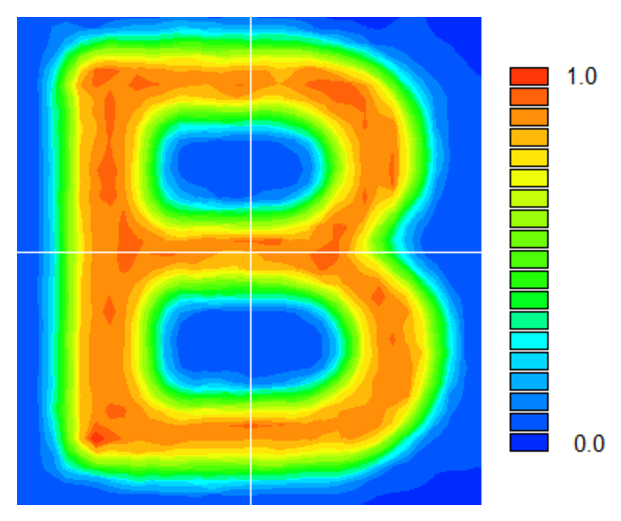
\includegraphics[width=0.35\textwidth]{app_letter_crop}
  \caption{Irradiance pattern as found by ray tracing for the case of
    an irrotational mapping}
  \label{fig:letterb}
\end{figure}

The integrability condition Eq.~\eqref{eq:integ} is computed with a
standard central difference scheme on a 3D discrete grid ($50\times 50
\times 3$ points) located in a $(x,y)$-plane close to the source
($z=10\mathrm{~mm}$) and with a vertical extent equal to the optics
size. Table~\ref{tab:map} shows the maximum absolute value and the RMS
of the curl for various configurations where one of the three parameters
$(1/T), R$ and $D$ has been progressively scaled up, the two others being 
held constant. All values are
given to three significant digits. The first line shows the value of
the curl using the initial values of the three parameters and a
non-optimized ray mapping (i.e. the starting mapping which still has a
significant curl). The second line corresponds to the initial value of
the geometrical parameters, but this time with the irrotational
mapping found using Eq.~\ref{eq:haker-ev}.  The improvement observed
(factor of about~60) confirms that the removal of the mapping's curl
provides a better adherence to the integrability condition
Eq.~\eqref{eq:integ}.  Finally, the three parameters are multiplied by
two (respectively four) and a corresponding reduction by a factor well
over two (respectively four) can be seen in the integrability
condition. This confirms the locally linear behavior expressed
in~\eqref{eq:map_quality}.


\subsection{Point source case}

In the case of a source point what follows shows that the reasoning still holds for  
small source emission angles only (which could also directly be stated
arguing  that this is close to the collimated case).
The author doesn't see yet a broader generalization.

\begin{figure}[!htbp]
  \centering 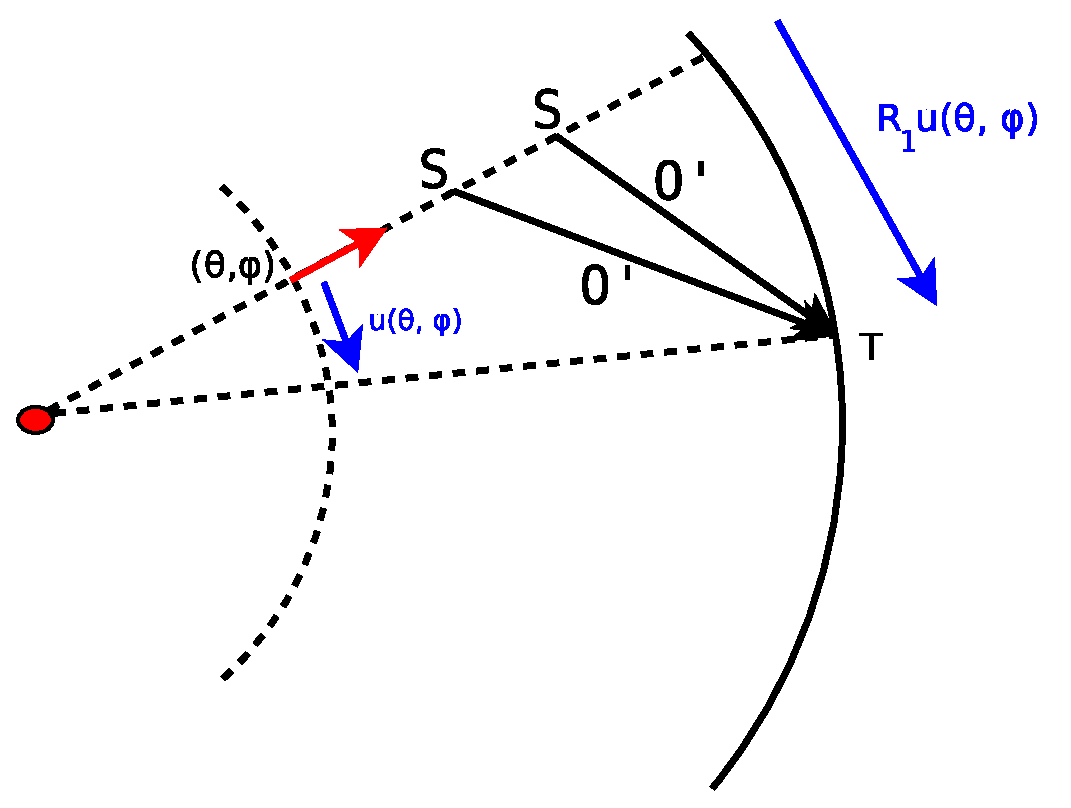
\includegraphics[width=0.45\textwidth]{appendix_sph}
  \caption{Point source configuration with a spherical
  coordinates parametrization. A ray is uniquely determined by the two angles $(\theta, \phi)$.  
  }
  \label{fig:appendix_sph}
\end{figure}

Switching to spherical coordinates.
The direct equivalent of the previous mapping is a function between
 two unit spheres (for example with $R=1$). That
is to say:
\[ \mathbf{A} : (\theta,\phi) \mapsto (t_\theta, t_\phi)\]

%To be able to apply Haker's equation, those two unit spheres are projected 
%in the code onto two planes $\Omega_0$ and $\Omega_1$ with a given projection
% $\mathbf{p}$
%(typically at present, a stereographic projection):
%\[ \mathbf{p}: (\theta, \phi) \mapsto (\rho, \phi)\]
%with $(\rho, \phi)$ the polar parametrization of the plane.
%
%For an arbitrary point $\s(\theta, \phi, r)$ in between the source and the target sphere,
%the point to be reached according to mapping is then:
%\[ T(\theta, \phi, R_1) = R_1 \mathbf{\tilde{u}}(\theta, \phi) + R_1 \mathbf{e}_r\]
%with $R_1$ the fixed radius of the target sphere (note the multiplication by $R_1$
%this time to account for the  bigger radius of the target).
%Consequently:
%\[ \Op = \T - \s = R_1\mathbf{\tilde{u}}(\theta, \phi) + (R_1-r)  \mathbf{e}_r\]
%or equivalently:
%\[ \Op = \T - \s = R_1\mathbf{p}^{-1}\left[ \mathbf{{u}} (\mathbf{p}(\theta, \phi)) \right]
% + (R_1-r)  \mathbf{e}_r\]
%
%With a spherical parametrization a point $\s(r, \theta, \phi)$ in 3D is associated
%uniquely to a point in a plane $\tilde{\s}$ with polar coordinates $\tilde{\s}(p(\theta), \phi)$.
%We assume indeed that the projection from the unit sphere to the plane conserves
%the azimuthal angle.

On the other side the 2D Haker's mapping writes with a polar parametrization:
\[ \mathbf{u}: (\rho, \phi) \mapsto (u_\rho(\rho, \phi), u_\phi(\rho, \phi)) \]
where $\rho$ is the polar radius and $\phi$ the polar angle.
This 2D function is once again made irrotational (with the same procedure)
 which in polar coordinates means (see Appendix):
\[ u_\phi + \rho\pderiv{u_\phi}{\rho} - \pderiv{u_\rho}{\phi} = 0 \]

The link between $\mathbf{u}$ and $\mathbf{A}$ is the projection from the 
unit sphere into the plane. We assume this projection to be rotation symmetric and hence
we write:
\[ p :\theta  \mapsto \rho \]

If the target is a sphere located at $r=R_1$ the light has to reach the point:
\[ \T(R_1, \theta, \phi) = R_1 \mathbf{A}(\theta, \phi) + R_1\mathbf{e}_r \]
with the field $\mathbf{A}$ being the mapping field linked to the 2D Haker's field
by the following relationships:
\begin{eqnarray*}
A_r &=& 0  \\
A_\theta &=& q[u_\rho(p(\theta),  \phi)]  =  q[u_\rho(\p)]  \\
A_\phi &=& u_\phi(p(\theta),  \phi)  = u_\phi(\p)
\end{eqnarray*}
where $p$ is the rotation-symmetric 
projection mentioned above,
and $q$ is its inverse. Furthermore $\p$ is
the projected point in the Haker's plane with radial coordinates
$ (\rho, \phi) = (p(\theta), \phi)$.

As for the collimated case the non-normalized field $\Op$ is still written:
\[ \Op = \T - \s \]
and computing the curl of $\Op$ amouts to compute the curl of $\mathbf{A}$.
We will need the following partial derivatives:
\begin{eqnarray*}
\pderiv{A_\phi}{\theta} &=& p'(\theta)\pderiv{u_\phi}{\rho}(\p)\\
\pderiv{A_\theta}{\phi} &=& \pderiv{u_\rho}{\phi}(\p)q'[u_\rho(\p)] 
\end{eqnarray*}

The formula of the curl in spherical coordinates (see appendix) result in
the following angular curl components:
\begin{eqnarray*}
C_\theta &=& -A_\phi / r = -u_\phi(\p) /r \\
C_\phi &=& A_\theta /r  = q[u_\rho(\p)] /r
\end{eqnarray*}

The last term of the curl along the radial direction is the tricky one:
\begin{eqnarray*}
C_r &=& \frac{1}{r\sin(\theta)} \left[ \sin(\theta) \pderiv{A_\phi}{\theta} +
   \cos(\theta) A_\phi - \pderiv{A_\theta}{\phi} \right] \\
& =& \frac{1}{r\sin(\theta)} \left[ \sin(\theta) p'(\theta)\pderiv{u_\phi}{\rho}(\p)
    + \cos(\theta) u_\phi(\p) - \pderiv{u_\rho}{\phi}(\p)q'[u_\rho(\p)] \right]  \\
\end{eqnarray*}

Assuming that: (a) $\theta$ remains small enough, and (b) that $p$ is such that its 
derivative close to the origin is equal to one (this last assumption is
not very strong and easy to satisfy), we can write:
\begin{eqnarray*}
\sin\theta &\simeq \theta \\
\cos\theta &\simeq 1 \\
p'(\theta) = q'[u_\rho(\p)] &\simeq 1
\end{eqnarray*}
hence leading to:
\[ C_r \simeq \frac{1}{r\sin(\theta)} \left[ \rho \pderiv{u_\phi}{\rho}(\p)
    +  u_\phi(\p) - \pderiv{u_\rho}{\phi}(\p) \right]  \simeq 0\]

If this last term is considered null, the curl of $\Op$ is perpendicular to $\I$
(it has only ortho-radial components) and
the same computation as before can be performed.

%We know that the curl of $\mathbf{u}(\rho, \phi)$ is null (Haker), but it is far
%from obvious that this holds when composing with~$\mathbf{p}$ and its inverse.

%However if $p =\, $Id, the reasoning should still hold (\red{TBC numerically - Adrien}).
%The limiting term would then write:
%\[ C \propto \frac{T_\theta}{R_\theta Z}\]
%with $T_\theta$ the \textit{angular} extent of the target (as seen from the source)
%and $R_\theta$ the \textit{angular} extent of the optics (typically $\theta_{max}$
%in the code).
%The limiting term remains locally approximated by:
%\[ C \propto \frac{T}{R Z}\]


%\textbf{TODO: if this is is correct, this would mean the stereographic 
%projection is to be reviewed - we should perform
%a much more simple projection: $(\theta, \phi) \mapsto (r = \theta, \phi)$. 
%\red{Wrong} - we simply need a projection which is linear at the origin
%}
%
%Numerical results computed with this projection: see table \ref{tab:map_point}

%\begin{table*}[!htbp]
%\centering
%\begin{tabular}{cc|c|c||c|c|c|}
%\cline{2-7}
% &  \multicolumn{6}{|c|}{Integrability condition ($\times 10^{-3}\,mm^{-1}$)} \\
%  \cline{2-7}
%\multicolumn{1}{c|}{} & \multicolumn{3}{c||}{Max} & \multicolumn{3}{c|}{RMS} \\ 
%\cline{2-7}
%\multicolumn{1}{c|}{} & 1/T & R & Z & 1/T & R & Z \\  \cline{2-7}
%\hline 
%\multicolumn{1}{|c|}{No mapping optimization} & \multicolumn{3}{c||}{657} & 
%\multicolumn{3}{c|}{205} \\ 
%\hline 
%\multicolumn{1}{|c|}{Optimized mapping} & \multicolumn{3}{c||}{20.6} & 
%\multicolumn{3}{c|}{4.94} \\ 
%\hline 
%\multicolumn{1}{|c|}{Parameter +25\%} & 12.1 &  10.4 & 12.0  & 3.26 & 3.32 & 3.20 \\ 
%\hline 
%\multicolumn{1}{|c|}{Parameter +50\%} & 9.96 &  7.64 & 9.40 & 3.16 & 2.57  &  2.88 \\ 
%\hline 
%\end{tabular}
%\caption{Integrability condition for various geometrical configurations in a point source run}
%\label{tab:map_point}
%\end{table*} 
%
%Doesn't hold when scaling the parameters by $\times 2$ or $\times 4$, confirming
%the local aspect of the ratio given previously.
%However we still observe that the linear estimation is a conservative one.
%\red{wrong interpretation after what precedes ...}

\subsection{General case}

errr ? still relevant ? we virtually handled all null étendue sources

\subsection{Multiple freeform surfaces}

tough one

